\documentclass[a4paper, 12pt]{article}
\usepackage{graphicx} % Required for inserting images
\usepackage{fullpage}
\usepackage{amsmath}
\usepackage{xcolor}
\usepackage{float}
\usepackage{geometry}
\usepackage{biblatex}
\geometry{margin=1in}
\usepackage{enumitem}
\usepackage{hyperref}
\usepackage{microtype}
\usepackage{parskip}

\title{M3 Math Test Study Guide}
\author{Rachel He}
\date{January 13, 2025}

\begin{document}

\maketitle

\subsection*{What decimal number is illustrated?}
Learn how to:

\begin{itemize}
    \item Read models divided into 10 and 100 squares and know their respective values
    \item Know that 1 row/column of the 100s model = 10 squares for easy counting
    \item Know whether to put shaded portions over 10 or 100 depending on the model shown
\end{itemize}

\textcolor{blue}{\textbf{Example 1}: Complete the problem below.}

\begin{figure}[H]
    \centering
    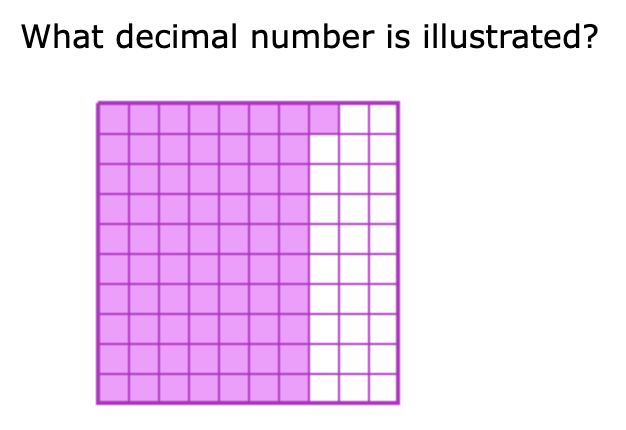
\includegraphics[width=0.5\linewidth]{dec.png}
    \label{fig:1}
\end{figure}

\subsection*{Compare decimals using models}

\textcolor{blue}{\textbf{Example 2}: Complete the problem below.}

\begin{figure}[H]
    \centering
    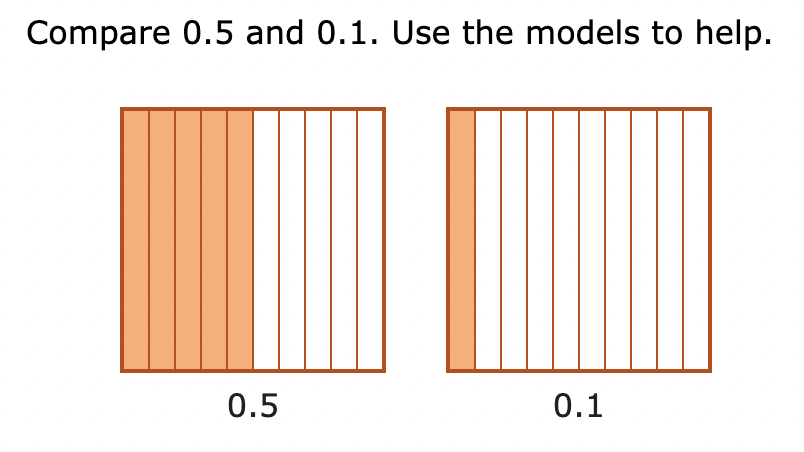
\includegraphics[width=0.5\linewidth]{comp.png}
    \caption{Caption}
    \label{fig:enter-label}
\end{figure}

\subsection*{Fractions with denominators of 10 and 100}

Learn how to:

\begin{itemize}
    \item Convert fractions with denominators of 10 into fractions with denominators of 100, and vice versa
\end{itemize}

\textcolor{blue}{\textbf{Example 3}: $\frac{3}{10}$ is equivalent to which fraction with 100 as its denominator?}

\subsection*{Comparing decimals}
Learn how to:

\begin{itemize}
    \item Compare decimals using your knowledge about place value
\end{itemize}

\textcolor{blue}{\textbf{Example 4}: Compare the decimals 0.56 and 0.5609.}

\newpage

\subsection*{Example Answers}

\paragraph{\textcolor{blue}{Example 1}} You have 2 ways of going about this: counting the shaded region and counting the unshaded region. Counting the unshaded region might be faster, but it requires subtracting from 100, so we'll go both ways.

We know by the look of the model that it's a 100s model, and each column contains 10 squares. Counting columns is easier than counting individual squares, so we can easily count 7 columns plus one additional square, giving us 71 out of 100 squares shaded, or $\boxed{\frac{71}{100}}$. In contrast, counting the number of unshaded squares, you get 20 plus 9 additional squares, and subtracting that from 100, you get the same answer.

\paragraph{\textcolor{blue}{Example 2}} You can tell from the models that 0.5 is greater than 0.1 since 5 bars are shaded on the left and only 1 on the right. So, the answer is $\boxed{0.5>0.1}$.

\paragraph{\textcolor{blue}{Example 3}} To get from 10 to 100, you multiply by 10; if you multiply the top by 10 also, you will have multiplied by $\frac{10}{10}$, which equals 1 and gives you an equivalent answer. The answer is $\boxed{\frac{30}{100}}$.

\paragraph{\textcolor{blue}{Example 4}} Looking at 0.56 and 0.5609, we can see that the tenths and hundredths place are identical. To tell which is greater, we take 0.56 out to 2 more decimal places: 0.5600. Since 0.5609 has a 9 in the ten thousandths place and 0.5600 has a 0, we can conclude that $\boxed{0.56<0.5609}$.

\end{document}
